\begin{abstract}
A six-layer CPU decoder was adapted to match clinical trial criteria to patient notes. Across 206 held-out annotations, accuracy rose from 22.8\% to 61.2\%, but the adapted model predicted just two categories and retrieved no evidence. This divergence makes accuracy alone misleading. Three decoding implementations returned identical tokens across three controlled workloads. A local browser application exposes the decisions, evidence gaps and runtime differences.
\end{abstract}
\begin{IEEEkeywords}trial screening, evidence retrieval, autoregressive decoding\end{IEEEkeywords}
\section{Introduction}
A recorded age can resolve an age threshold, but an unmentioned medication cannot resolve a contraindication. We ask whether an open CPU decoder can jointly generate a criterion judgment and the sentence IDs that support it. Trial-level summaries aggregate individual predictions by explicit rules. The annotations supply ground truth at criterion level.
\section{Related Work and Architecture}
TrialGPT separates trial retrieval, matching and ranking \cite{trial}. Supplying criteria directly isolates its matching task here. We compare against the same decoder before adaptation because the published TrialGPT results use another protocol. The Pythia suite supports controlled architectural investigation \cite{pythia}. Our two candidates are Apache-2.0 GPT-NeoX decoders with byte-level BPE and a 2,048-position context \cite{small,large}. Pythia-14M has six layers of width 128 and four heads. Pythia-70M has six wider layers of width 512 and eight heads. Nominal FP32 weight storage is roughly 56 versus 280 MB before gradients, optimizer state and activations. The smaller model was selected for repeated CPU runs. Its performance relative to 70M remains unmeasured.
LoRA reduces training state through low-rank updates \cite{lora}. Freezing the input embedding and selecting the output vocabulary here leaves about 1.20M trainable weights, allowing direct updates. FlashAttention tiles exact attention to reduce data movement \cite{flash}; this study tests its underlying recurrence independently. Speculative decoding amortizes target passes over draft proposals \cite{spec}. Short structured outputs restrict opportunities to recover drafting overhead.
\section{Materials and Methods}
\subsection{Patient-level split and structured prediction}
The NCBI benchmark \cite{data} contains 1,015 rows from 53 patients. Lexically sorted unique patient IDs were shuffled with NumPy default\_rng(42). The prescribed 37/8/8 patient groups contain 603/206/206 annotations. A separate check reconstructed the split, checked disjointness and accounted for every annotation. Only patient note, criterion type and criterion text enter the prompt. Expert labels and original sentence IDs are targets. GPT-generated columns and the legacy split flag are excluded. A missing training criterion is preserved with an explicit missing-text marker.
\begin{figure}[ht]\centering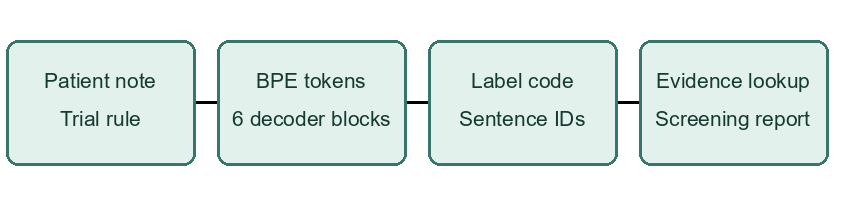
\includegraphics[width=\columnwidth]{workflow.png}\caption{Screening workflow from original text to reviewable output.}\label{fig:flow}\end{figure}
Figure~\ref{fig:flow} distinguishes prediction from verbatim sentence lookup. The decoder emits a label symbol, ascending unique sentence IDs and a stop symbol. Type and available sentence numbers constrain legal outputs. The 107-row head is initialized from corresponding pretrained output rows, avoiding a projection onto all 50,304 tokens. Before and after adaptation the same output grammar applies. The deployed network contains 7,642,496 parameters. Classification explanations describe the model judgment and indicate missing support.
\subsection{Training and model selection}
Training used four FP32 epochs on two CPU threads, Python and PyTorch seed 42, teacher-forced answer-only cross-entropy, AdamW at 0.0002, weight decay 0.01, accumulation over four records and gradient norm clipping at 1. The final partial batch also takes a step. The input embedding stays frozen. Prompt lengths peaked at 453/322/361 tokens across train/validation/test. No benchmark note was truncated; the app rejects inputs above 1,930 prompt tokens. The highest validation six-class macro-F1 selects the checkpoint, with earliest epoch winning ties. Its hash was recorded before final test scoring.
\begin{figure}[ht]\centering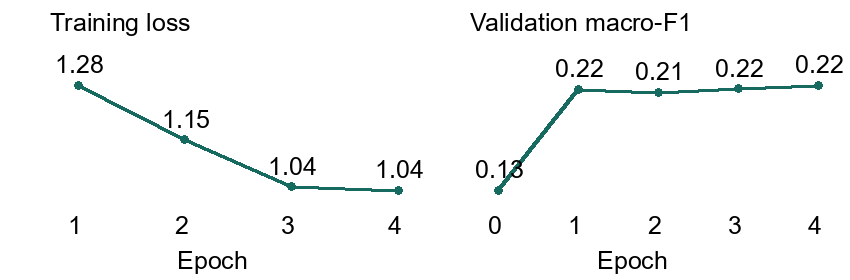
\includegraphics[width=\columnwidth]{training.png}\caption{Training loss and validation macro-F1. Epoch zero denotes the base decoder.}\label{fig:train}\end{figure}
Figure~\ref{fig:train} shows decreasing loss and a much smaller validation gain after epoch one. Epoch four reached 0.219 validation macro-F1.
\subsection{Decoding and attention}
Uncached inference recomputes the prefix. Cached inference stores rotated keys and values for each layer. The next token position equals the cached length, and the mask permits keys through the absolute query position. Shape-dependent rounding can affect a near-tied argmax. The draft uses the first two pretrained blocks and the same tokenizer and restricted head vocabulary. It proposes up to four tokens. One target pass verifies a block. On rejection both caches are sliced to the accepted prefix and the corrected target token remains pending. Full agreement permits an extra target token.
Reference attention applies stable row softmax to scaled query-key dot products after masking. Each query tile instead maintains maximum $m$, denominator $z$ and numerator $a$. Given scores $S$, let $m'=\max(m,\max S)$ and $P=\exp(S-m')$. Update $z'=e^{m-m'}z+\sum P$ and $a'=e^{m-m'}a+PV$, then divide the final $a$ by $z$. Blocks have width 32. Wholly future blocks are skipped; partial blocks use absolute causal offsets. This educational kernel is tested separately. The deployed decoder uses PyTorch scaled dot-product attention.
\section{Experimental Setup and Metrics}
Experiments used an HP EliteBook 840 G8 with 15.7 GiB RAM and CPU-only PyTorch 2.8.0. The validation reference audit compared restricted logits against the official Transformers implementation at 5, 32 and 96 positions. All 133 argmax decisions agreed. Maximum absolute logit difference was 0.00246; the custom path uses a different residual addition order and attention implementation. Cached versus full-prefix chunk checks had a maximum absolute difference of 0.000059 and identical argmax tokens. Accuracy and macro-F1 use fixed class sets (six overall and four by type). Undefined class scores are zero. Evidence micro scores pool overlaps and set sizes; macro scores average per-record precision, recall and F1. Two empty sets receive one for each per-record score. A one-sided empty denominator receives zero. Benchmark prompts use validation prefixes and controlled fixed output budgets, with stop disabled. Each CPU timing uses a warm-up and median of five synchronous repetitions. Sampled process RSS includes the interpreter, both models and allocator. It can miss short-lived peaks. Prefill and decode medians are timed separately.
\section{Results and Discussion}
\begin{table}[t]\centering\caption{All adaptation runs, validation split only (best epoch by the selection score)}\label{tab:runs}\footnotesize
\begin{tabular}{lrrrrrr}
\hline
Configuration & Ep. & Best & Acc. & MF1$_p$ & Ev.F1 & Sel.\\\hline
14M, unw. (1st subm.), 2e-4, 4\,ep & 4 & 4 & 0.621 & 0.219 & 0.000 & 0.109\\
14M, bal.\,$p{=}$0.5, ev+stop $\times$3, 3e-4 & 3 & 1 & 0.621 & 0.215 & 0.000 & 0.108\\
14M, unw., ev+stop $\times$3, 3e-4 & 3 & 1 & 0.621 & 0.215 & 0.000 & 0.108\\
14M, bal.\,$p{=}$0.5, ev $\times$5, 3e-4 & 6 & 3 & 0.617 & 0.213 & 0.017 & 0.115\\
14M, bal.\,$p{=}$0.5, ev $\times$5, 1e-3 & 6 & 5 & 0.626 & 0.218 & 0.000 & 0.109\\
70M, bal.\,$p{=}$1, ev $\times$5, 2e-4, 10\,ep & 10 & 10 & 0.650 & 0.328 & 0.250 & 0.289\\
70M, bal.\,$p{=}$1, ev $\times$5, 2e-4, 16\,ep & 16 & 9 & 0.631 & 0.277 & 0.360 & 0.318\\
\hline\end{tabular}
\\[2pt]\parbox{0.98\linewidth}{\scriptsize ``ev+stop'' runs used an early weighting bug that also up-weighted the stop symbol; 14M runs were stopped early once collapse was evident. The last row is the frozen model.}
\end{table}

\begin{table}[t]\centering\caption{Latent signal on validation from teacher-forced logits (ROC-AUC; 0.5 = chance)}\label{tab:diag}\footnotesize
\begin{tabular}{lrrrr}
\hline
Model & Mean label & Included & Excl. N/A & Evidence\\\hline
Pythia-14M base & 0.56 & 0.61 & 0.29 & 0.46\\
Pythia-14M 1st subm. & 0.46 & 0.52 & 0.44 & 0.66\\
Pythia-70M base & 0.55 & 0.56 & 0.48 & 0.51\\
Pythia-70M final & 0.53 & 0.71 & 0.74 & 0.69\\
\hline\end{tabular}
\end{table}

\begin{table}[t]\centering\caption{Fine-tuning configuration (Pythia-70M target)}\label{tab:hparams}\footnotesize
\begin{tabular}{ll}
\hline
Setting & Value\\\hline
Trainable / total parameters & 18,970,112 / 44,725,760\\
Frozen & input embedding (25.8M)\\
Objective & answer-only teacher-forced CE\\
Label weights & balanced, power 1\\
Evidence-ID weight & 5 (stop symbol 1)\\
Optimiser & AdamW, wd 0.01, clip 1.0\\
Learning rate & 0.0002, 6\% warm-up, linear decay\\
Batch & 1 record, accumulate 4\\
Epochs / selected & 16 / 9\\
Precision / threads / seed & FP32 / 6 CPU / 42\\
\hline\end{tabular}
\end{table}

\begin{table*}[t]\centering\caption{Paired before/after comparison on identical validation and held-out test rows (constrained greedy decoding)}\label{tab:scores}\footnotesize
\begin{tabular}{llcccccccccc}
\hline
Split & System & Acc. & MF1$_6$ & MF1$_p$ & Acc$_{inc}$ & Acc$_{exc}$ & Ev.P & Ev.R & Ev.F1$_\mu$ & Ev.F1$_M$ & Ev.F1$_M^{+}$\\\hline
Validation & Majority & 0.621 & 0.215 & 0.215 & 0.409 & 0.721 & 0.000 & 0.000 & 0.000 & 0.563 & 0.000\\
Validation & Maj.+lead sent. & 0.621 & 0.215 & 0.215 & 0.409 & 0.721 & 0.204 & 0.365 & 0.262 & 0.178 & 0.407\\
Validation & 1st subm. 14M & 0.621 & 0.219 & 0.219 & 0.409 & 0.721 & 0.000 & 0.000 & 0.000 & 0.563 & 0.000\\
Validation & Base 70M & 0.209 & 0.147 & 0.147 & 0.530 & 0.057 & 0.102 & 0.078 & 0.089 & 0.468 & 0.071\\
Validation & Adapted (final) & 0.631 & 0.277 & 0.277 & 0.409 & 0.736 & 0.459 & 0.296 & 0.360 & 0.602 & 0.334\\
Test & Majority & 0.626 & 0.226 & 0.272 & 0.507 & 0.695 & 0.000 & 0.000 & 0.000 & 0.704 & 0.000\\
Test & Maj.+lead sent. & 0.626 & 0.226 & 0.272 & 0.507 & 0.695 & 0.184 & 0.404 & 0.253 & 0.150 & 0.508\\
Test & 1st subm. 14M & 0.612 & 0.222 & 0.266 & 0.507 & 0.672 & 0.000 & 0.000 & 0.000 & 0.704 & 0.000\\
Test & Base 70M & 0.194 & 0.144 & 0.173 & 0.360 & 0.099 & 0.099 & 0.149 & 0.119 & 0.549 & 0.083\\
Test & Adapted (final) & 0.631 & 0.279 & 0.334 & 0.507 & 0.702 & 0.315 & 0.245 & 0.275 & 0.635 & 0.340\\
\hline\end{tabular}
\\[2pt]\parbox{0.95\linewidth}{\scriptsize MF1$_6$: macro-F1 over all six labels (zero-support classes count as 0); MF1$_p$: over labels present in the gold set. Ev.\ = evidence sentence retrieval; $\mu$ micro (pooled), $M$ per-record macro where two empty sets score 1, $M^{+}$ macro over records with non-empty gold evidence only. Majority = type-conditioned training majority label without evidence; Maj.+lead sent.\ adds the first note sentence as evidence; 1st subm.\ = our original Pythia-14M submission re-scored with these metrics.}
\end{table*}

\begin{table}[t]\centering\caption{Adapted model, held-out test, inclusion criteria ($n=75$): per-class scores and confusion matrix (rows gold, columns predicted)}\label{tab:cls_inclusion}\footnotesize
\begin{tabular}{lrccc|rrrr}
\hline
Gold & n & P & R & F1 & Incl. & Not incl. & NEI & N/A\\\hline
Incl. & 27 & 0.000 & 0.000 & 0.000 & 0 & 0 & 27 & 0\\
Not incl. & 7 & 0.000 & 0.000 & 0.000 & 0 & 0 & 7 & 0\\
NEI & 38 & 0.507 & 1.000 & 0.673 & 0 & 0 & 38 & 0\\
N/A & 3 & 0.000 & 0.000 & 0.000 & 0 & 0 & 3 & 0\\
\hline\end{tabular}
\end{table}

\begin{table}[t]\centering\caption{Adapted model, held-out test, exclusion criteria ($n=131$): per-class scores and confusion matrix (rows gold, columns predicted)}\label{tab:cls_exclusion}\footnotesize
\begin{tabular}{lrccc|rrrr}
\hline
Gold & n & P & R & F1 & Excl. & Not excl. & NEI & N/A\\\hline
Excl. & 0 & 0.000 & 0.000 & 0.000 & 0 & 0 & 0 & 0\\
Not excl. & 91 & 0.706 & 0.978 & 0.820 & 0 & 89 & 1 & 1\\
NEI & 28 & 0.000 & 0.000 & 0.000 & 0 & 28 & 0 & 0\\
N/A & 12 & 0.750 & 0.250 & 0.375 & 0 & 9 & 0 & 3\\
\hline\end{tabular}
\end{table}

\begin{table}[t]\centering\caption{Held-out test per-label F1 and prediction counts before (base) and after adaptation}\label{tab:classes}\footnotesize
\begin{tabular}{lrcccc}
\hline
Label & Support & F1 base & F1 adapt. & \#pred base & \#pred adapt.\\\hline
Incl. & 27 & 0.529 & 0.000 & 75 & 0\\
Not incl. & 7 & 0.000 & 0.000 & 0 & 0\\
Excl. & 0 & 0.000 & 0.000 & 87 & 0\\
Not excl. & 91 & 0.000 & 0.820 & 0 & 126\\
NEI & 66 & 0.224 & 0.535 & 41 & 76\\
N/A & 15 & 0.111 & 0.316 & 3 & 4\\
\hline\end{tabular}
\end{table}

\begin{table*}[t]\centering\caption{Test difference of the adapted model with patient-level 95\% bootstrap intervals (5000 resamples of the 8 test patients)}\label{tab:ci}\footnotesize
\begin{tabular}{lccc}
\hline
Adapted & $\Delta$Acc. & $\Delta$MF1$_p$ & $\Delta$Ev.F1$_\mu$\\\hline
vs.\ majority & +0.005 [-0.012, +0.020] & +0.062 [+0.000, +0.130] & +0.275 [+0.181, +0.368]\\
vs.\ maj.+lead & +0.005 [-0.012, +0.020] & +0.062 [+0.000, +0.130] & +0.022 [-0.063, +0.106]\\
vs.\ base 70M & +0.437 [+0.163, +0.646] & +0.161 [+0.013, +0.315] & +0.156 [+0.056, +0.326]\\
\hline\end{tabular}
\\[2pt]\parbox{0.95\linewidth}{\scriptsize Exact McNemar test on label correctness, adapted vs.\ majority: 3 vs.\ 2 discordant criteria, $p=1.00$.}
\end{table*}

\begin{table*}[t]\centering\caption{Controlled greedy decoding on the adapted 70M target (stop suppressed; warm-up + median of 5; CPU, 2 threads)}\label{tab:runtime}\footnotesize
\begin{tabular}{llrrrrrrrrc}
\hline
In/out & Path & Prefill & Decode & Total ms & Tok/s & $\times$unc. & RSS MiB & KV KiB & Acc./prop. & Equal\\\hline
32/8 & uncached & 21.1 & 169.7 & 190.8 & 41.9 & 1.00 & 643 & -- & -- & yes\\
32/8 & cached & 22.2 & 43.2 & 65.3 & 122.4 & 2.92 & 643 & 960 & -- & yes\\
32/8 & speculative (early-exit) & -- & -- & 161.5 & 49.5 & 1.18 & 618 & -- & 0/26 & yes\\
32/8 & speculative (14M) & -- & -- & 77.9 & 102.7 & 2.52 & 618 & -- & 7/7 & yes\\
256/32 & uncached & 82.3 & 2791.5 & 2873.8 & 11.1 & 1.00 & 678 & -- & -- & yes\\
256/32 & cached & 90.2 & 218.1 & 308.2 & 103.8 & 9.32 & 677 & 6912 & -- & yes\\
256/32 & speculative (early-exit) & -- & -- & 336.1 & 95.2 & 8.55 & 657 & -- & 22/40 & yes\\
256/32 & speculative (14M) & -- & -- & 704.0 & 45.5 & 4.03 & 664 & -- & 7/98 & yes\\
1024/64 & uncached & 387.5 & 24756.7 & 25144.2 & 2.5 & 1.00 & 810 & -- & -- & yes\\
1024/64 & cached & 395.2 & 665.4 & 1060.6 & 60.3 & 23.71 & 806 & 26112 & -- & yes\\
1024/64 & speculative (early-exit) & -- & -- & 1124.9 & 56.9 & 22.35 & 799 & -- & 45/74 & yes\\
1024/64 & speculative (14M) & -- & -- & 2143.7 & 29.9 & 11.85 & 785 & -- & 12/205 & yes\\
\hline\end{tabular}
\\[2pt]\parbox{0.95\linewidth}{\scriptsize Prefill and decode are timed separately for the two non-speculative paths; speculative time is end-to-end (both prefills included). KV KiB is the analytic FP32 cache size at the end of generation. RSS is sampled process memory (interpreter, all models) and can miss short peaks. Equal: token sequence identical to the uncached reference.}
\end{table*}

\begin{table}[t]\centering\caption{Real screening outputs (grammar and stop enabled) on 24 validation criteria: mean latency per criterion}\label{tab:screening}\footnotesize
\begin{tabular}{lrrrrrr}
\hline
Path & n & Mean ms & Out tok. & Accepted & Rate & Equal\\\hline
uncached & 24 & 184.5 & 2.33 & -- & -- & 24/24\\
cached & 24 & 88.4 & 2.33 & -- & -- & 24/24\\
speculative (early-exit) & 24 & 131.7 & 2.33 & 24/104 & 23\% & 24/24\\
speculative (14M) & 24 & 106.0 & 2.33 & 55/57 & 96\% & 24/24\\
\hline\end{tabular}
\end{table}

\begin{table*}[t]\centering\caption{Attention kernels vs.\ an FP64 SDPA ground truth (4 heads, $d_h=32$, FP32, median of 5)}\label{tab:attention}\footnotesize
\begin{tabular}{lccrrrrrrrr}
\hline
$L_q\times L_k$ & C & Blk & Ref max & Tiled max & Tiled mean & Ref ms & Tiled ms & SDPA ms & Full KiB & Tile KiB\\\hline
17$\times$17 & y & 32 & 5.4e-07 & 5.4e-07 & 4.1e-08 & 0.22 & 0.39 & 0.07 & 5 & 5\\
17$\times$17 & n & 32 & 5.4e-07 & 5.4e-07 & 4.5e-08 & 0.15 & 0.25 & 0.06 & 5 & 5\\
65$\times$65 & y & 32 & 4.7e-07 & 5.0e-07 & 3.5e-08 & 0.31 & 1.43 & 0.13 & 66 & 16\\
65$\times$65 & n & 32 & 3.8e-07 & 3.8e-07 & 3.1e-08 & 0.20 & 1.43 & 0.09 & 66 & 16\\
256$\times$256 & y & 32 & 6.1e-07 & 6.1e-07 & 2.6e-08 & 1.45 & 7.35 & 0.59 & 1024 & 16\\
256$\times$256 & n & 32 & 3.5e-07 & 2.6e-07 & 1.8e-08 & 0.52 & 10.09 & 0.47 & 1024 & 16\\
512$\times$512 & y & 32 & 6.7e-07 & 6.1e-07 & 2.1e-08 & 5.74 & 25.09 & 2.05 & 4096 & 16\\
512$\times$512 & n & 32 & 5.4e-07 & 2.6e-07 & 1.4e-08 & 2.39 & 36.24 & 1.31 & 4096 & 16\\
1$\times$300 & y & 32 & 7.0e-08 & 5.4e-08 & 1.4e-08 & 0.18 & 1.54 & 0.06 & 5 & 0\\
1$\times$300 & n & 32 & 7.0e-08 & 5.4e-08 & 1.4e-08 & 0.13 & 1.26 & 0.06 & 5 & 0\\
40$\times$300 & y & 32 & 2.4e-07 & 3.2e-07 & 1.9e-08 & 0.35 & 3.46 & 0.21 & 188 & 16\\
40$\times$300 & n & 32 & 2.8e-07 & 2.8e-07 & 1.9e-08 & 0.24 & 2.71 & 0.16 & 188 & 16\\
256$\times$256 & y & 8 & 6.1e-07 & 5.6e-07 & 2.6e-08 & 1.36 & 74.73 & 0.52 & 1024 & 1\\
256$\times$256 & y & 16 & 6.1e-07 & 5.4e-07 & 2.5e-08 & 1.44 & 20.73 & 0.55 & 1024 & 4\\
256$\times$256 & y & 64 & 6.1e-07 & 6.1e-07 & 2.7e-08 & 1.41 & 2.66 & 0.55 & 1024 & 64\\
256$\times$256 & y & 128 & 6.1e-07 & 6.1e-07 & 3.0e-08 & 1.27 & 1.40 & 0.57 & 1024 & 256\\
\hline\end{tabular}
\\[2pt]\parbox{0.95\linewidth}{\scriptsize Errors are maximum/mean absolute differences from FP64 \texttt{scaled\_dot\_product\_attention}. Full/Tile KiB: size of the score matrix materialised by the reference versus the largest single tile of the online-softmax kernel. Rectangular shapes ($L_q<L_k$) model decoding with a KV cache.}
\end{table*}

\subsection{Eight held-out errors}
Row 159 misses the explicitly recorded age of 67 and its citation. Row 161 assigns uncertainty to an elective carotid procedure experts marked not included; the note describes cardiac catheterization. Row 165 changes a not-applicable pregnancy criterion into not excluded. Row 169 clears a low-filtration exclusion without the numerical evidence required to resolve it. Row 179 predicts the expert catheterization label but omits sentence 0. Row 306 correctly signals uncertainty about liver resection but omits sentence 3 describing drainage of an abscess. Row 322 loses sex-related context in sentence 0 and changes the expert exclusion judgment to uncertainty. Row 422 misses the birth-control applicability judgment and sentence 3. Frequent labels and early termination after a label are plausible contributors; their causal roles remain untested.
\subsection{Browser application}
\begin{figure}[ht]\centering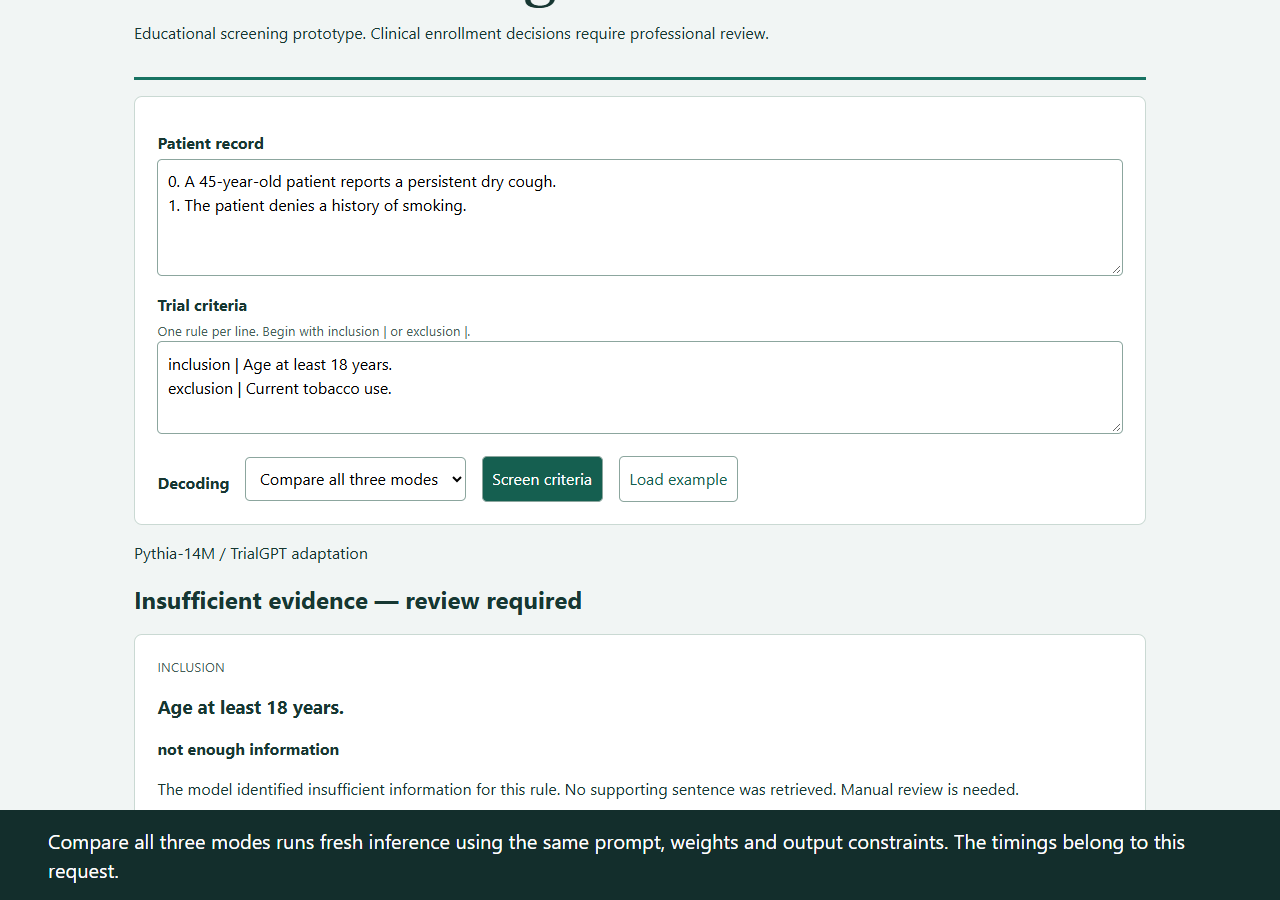
\includegraphics[width=\columnwidth]{application.png}\caption{Browser interface during the recorded local demonstration.}\label{fig:app}\end{figure}
Figure~\ref{fig:app} shows the local workflow. Comparison mode runs all three decoders on the entered criteria. Text export includes predictions, evidence and provenance. A cited failed inclusion or positive exclusion flags a potential conflict. Uncertainty or missing citations trigger review. Other cases report no flagged conflict among entered criteria. No trial-level outcome is treated as a benchmark label.
\section{Limitations and Conclusion}
Only eight patients contribute to the test metrics. Repeated criteria from a patient are correlated, and one class has zero support. Accuracy gains conceal loss of evidence retrieval. This model cannot support clinical enrollment decisions. Its reproducible contribution is a small experimental system that exposes these failures and tests whether alternative inference paths preserve the same outputs.
\section*{AI-use appendix}
OpenAI Codex assisted with planning, code, experiment execution, error analysis, report drafting and the captioned browser demonstration. The submission contains the measured outputs and checkpoint. The student is responsible for understanding the implementation and conducting the live defense.
\begin{thebibliography}{9}
\bibitem{trial} Q. Jin et al., Matching patients to clinical trials with large language models, Nature Communications, 2024, doi:10.1038/s41467-024-53081-z.
\bibitem{pythia} S. Biderman et al., Pythia: A suite for analyzing large language models across training and scaling, ICML, 2023.
\bibitem{small} EleutherAI, Pythia-14M model card and configuration. \url{https://huggingface.co/EleutherAI/pythia-14m}
\bibitem{large} EleutherAI, Pythia-70M model card and configuration. \url{https://huggingface.co/EleutherAI/pythia-70m}
\bibitem{lora} E. Hu et al., LoRA: Low-rank adaptation of large language models, ICLR, 2022.
\bibitem{flash} T. Dao et al., FlashAttention: Fast and memory-efficient exact attention with IO-awareness, NeurIPS, 2022.
\bibitem{spec} Y. Leviathan, M. Kalman and Y. Matias, Fast inference from transformers via speculative decoding, ICML, 2023.
\bibitem{data} NCBI, TrialGPT criterion annotations. \url{https://huggingface.co/datasets/ncbi/TrialGPT-Criterion-Annotations}
\end{thebibliography}

